\section{Planning + Learning}
\frame{\tableofcontents[currentsection, hideothersubsections]}

\begin{frame}
\frametitle{Planning, Acting and Learning in MDP}
\begin{figure}
    \centering
    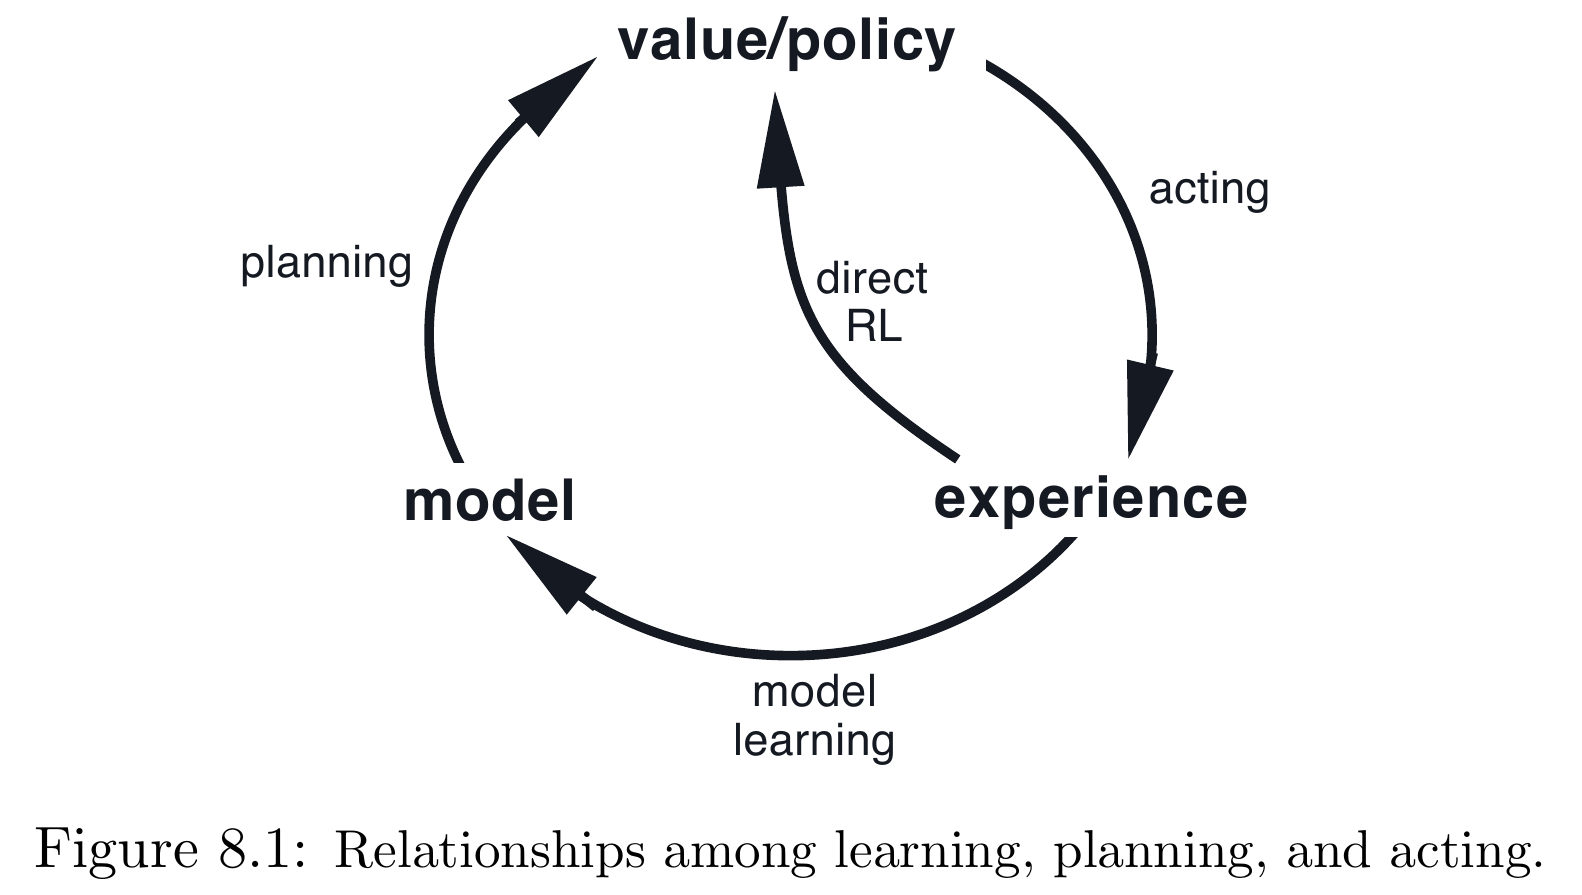
\includegraphics[scale=0.35]{learning_planning_acting_rl_intro_p176}
\end{figure}
\end{frame}

\begin{frame}
\frametitle{Planning vs direct Reinforcement Learning (Direct-RL)}
\begin{columns}
  \column{0.5\textwidth}
    \begin{figure}
        \centering
        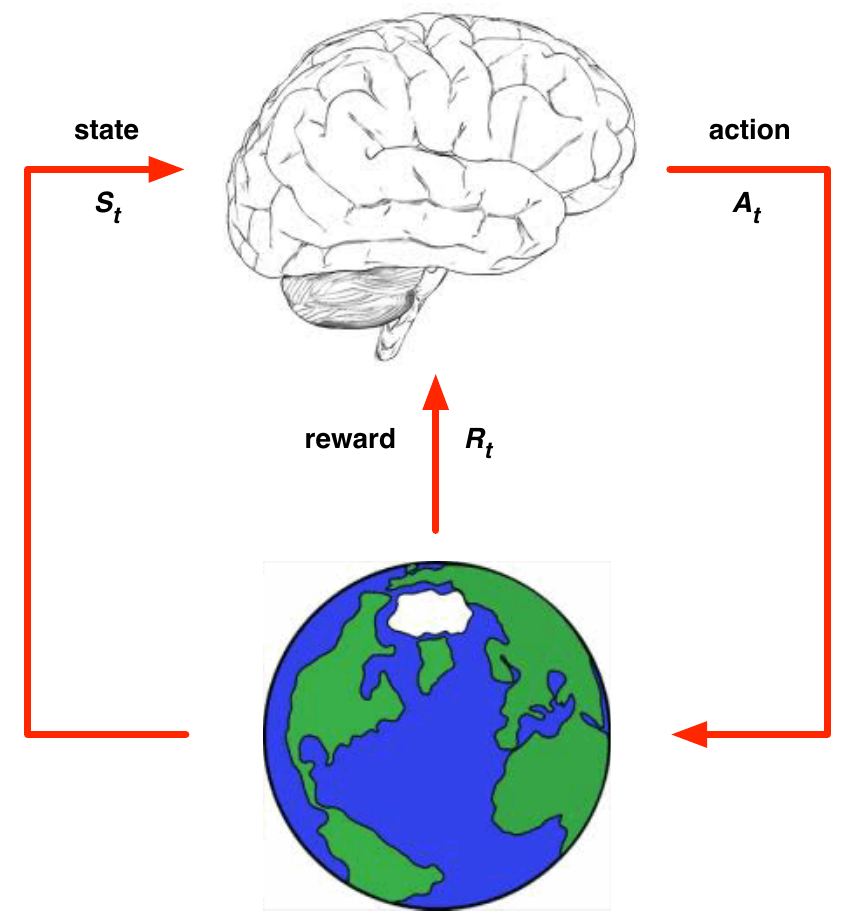
\includegraphics[scale=0.25]{model_based_silver_course}
        \caption{Planning uses a \textbf{model} env.}
    \end{figure}

  \column{0.5\textwidth}
    \begin{figure}
        \centering
        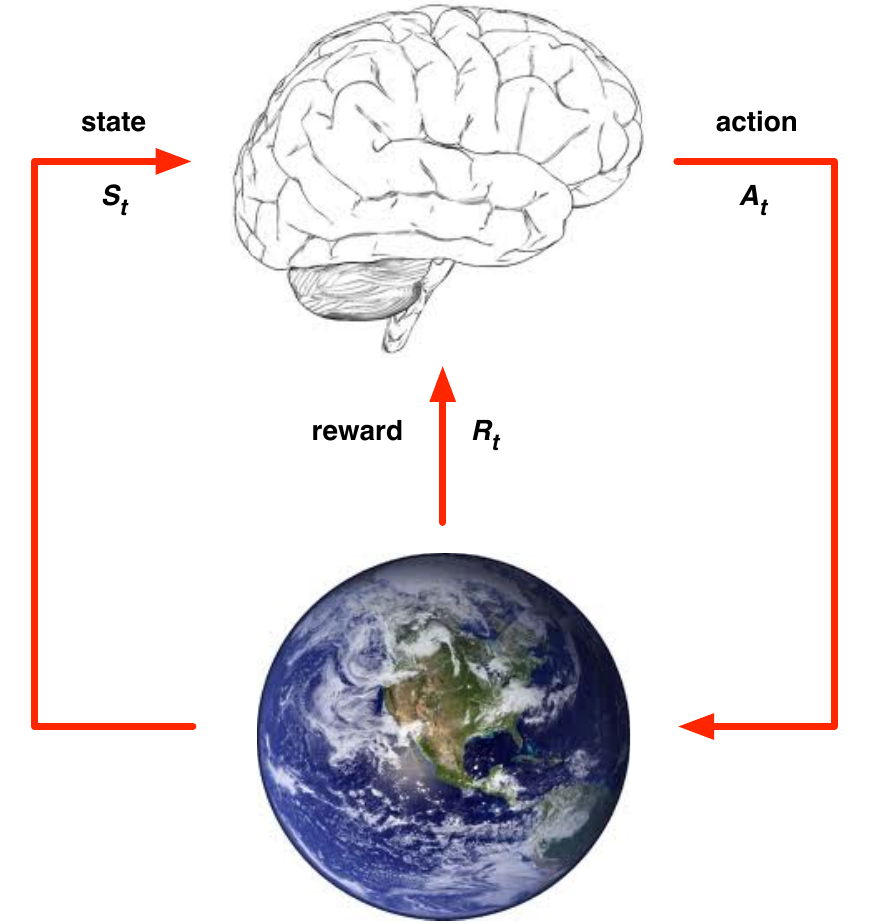
\includegraphics[scale=0.25]{model_free_silver_course}
        \caption{Direct-RL uses a \textbf{real} env.}
    \end{figure}
\end{columns}
\end{frame}

\begin{frame}
\frametitle{Planning vs direct Reinforcement Learning (Direct-RL)}
\begin{columns}
  \column{0.5\textwidth}
    \begin{figure}
        \centering
        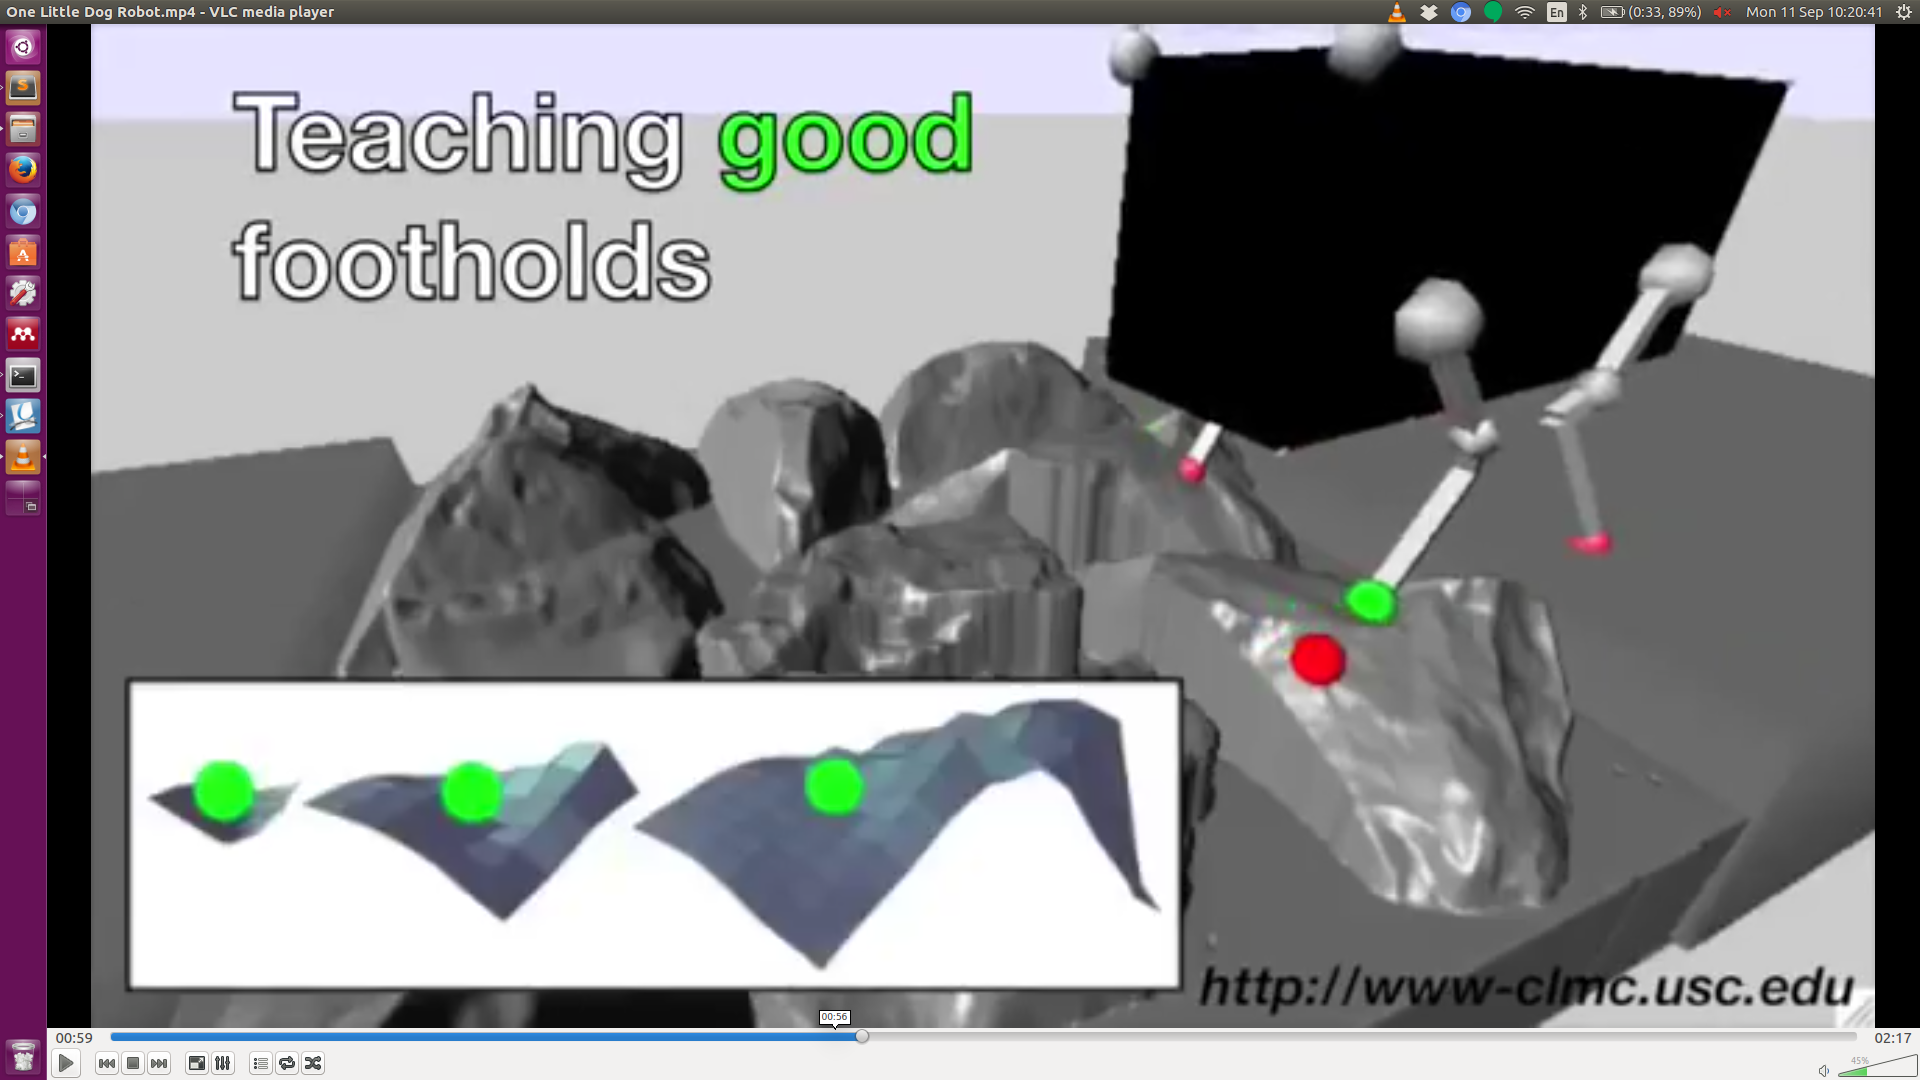
\includegraphics[scale=0.1]{little_dog_model_env}
        \caption{Planning uses a \textbf{model} env.}
    \end{figure}

  \column{0.5\textwidth}
    \begin{figure}
        \centering
        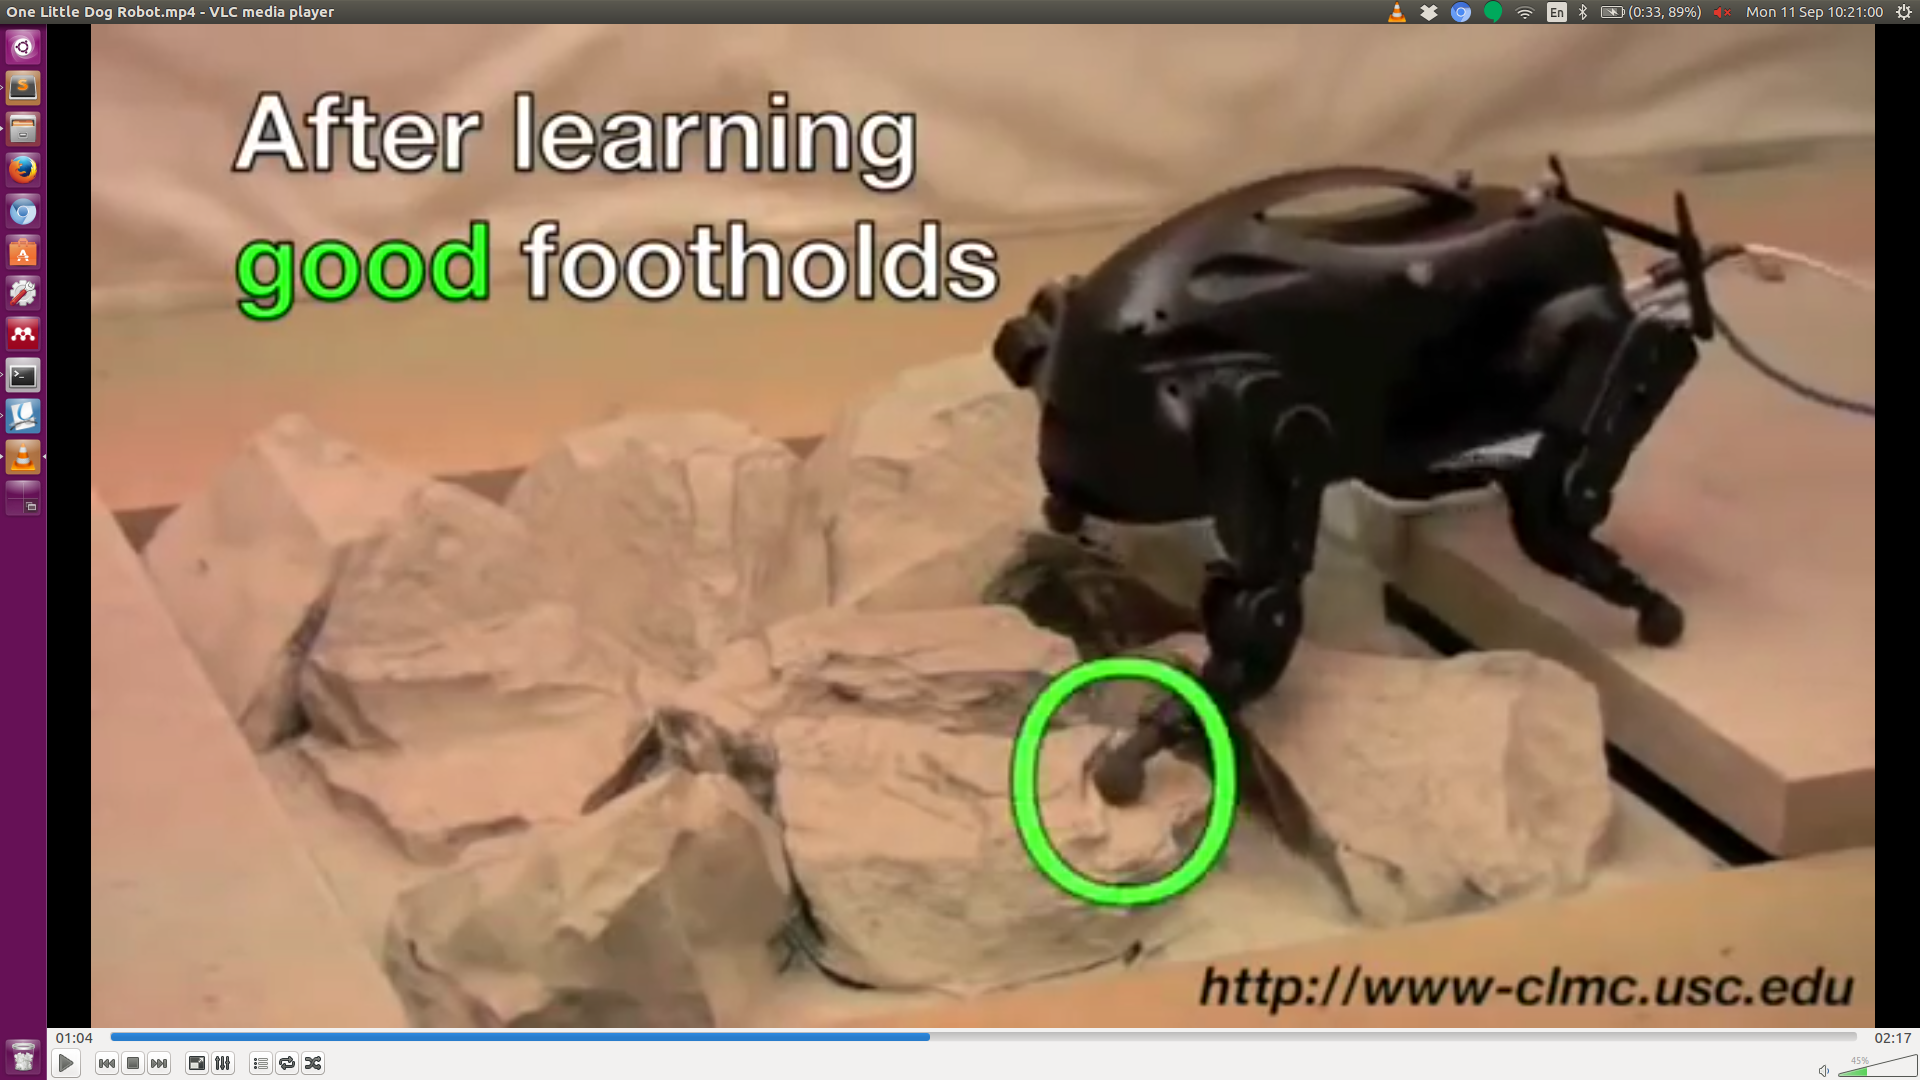
\includegraphics[scale=0.1]{little_dog_real_env}
        \caption{Direct-RL uses a \textbf{real} env.}
    \end{figure}
\end{columns}
\end{frame}

\begin{frame}
\frametitle{Q-learning for both planning and direct-RL}
\begin{figure}
    \centering
    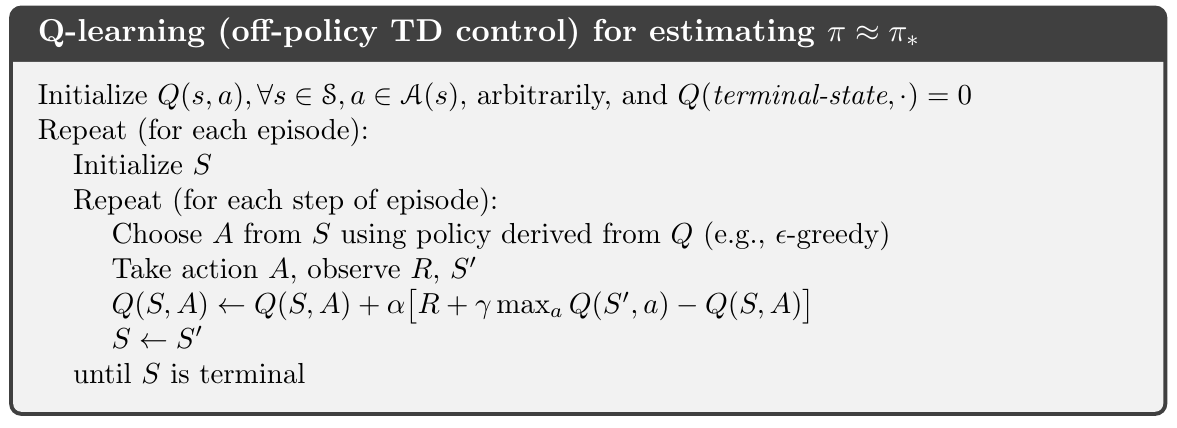
\includegraphics[scale=0.40]{q_learning_rl_intro_p142}
\end{figure}
\pause

\textbf{Action value-function} is the value of taking action $a$ in state $s$ \\
$Q(s,a) = \mathbb{E} [\sum_{k=0}^{\infty} \lambda^k~r_{t+k+1} | S_t = s, A_t = a]$\\
\noindent\rule{5cm}{0.4pt}\\
Note $Q:(s,a) \mapsto \mathbb{R}$,\\
\hspace{2mm} c.f $V: s \mapsto \mathbb{R}$
\pause

\end{frame}

\begin{frame}
\frametitle{Q-learning vs Value Iteration}
\begin{figure}
    \centering
    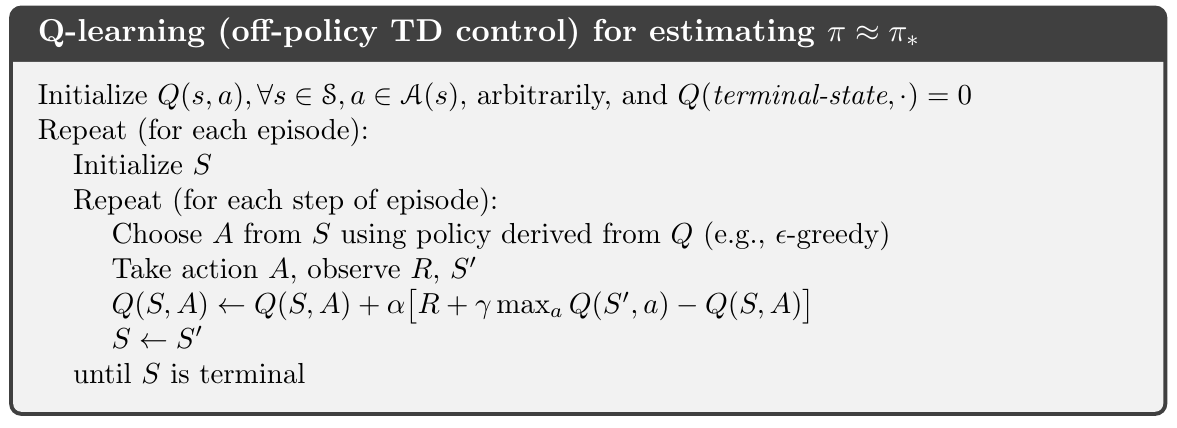
\includegraphics[scale=0.3]{q_learning_rl_intro_p142}
\end{figure}

\begin{figure}
    \centering
    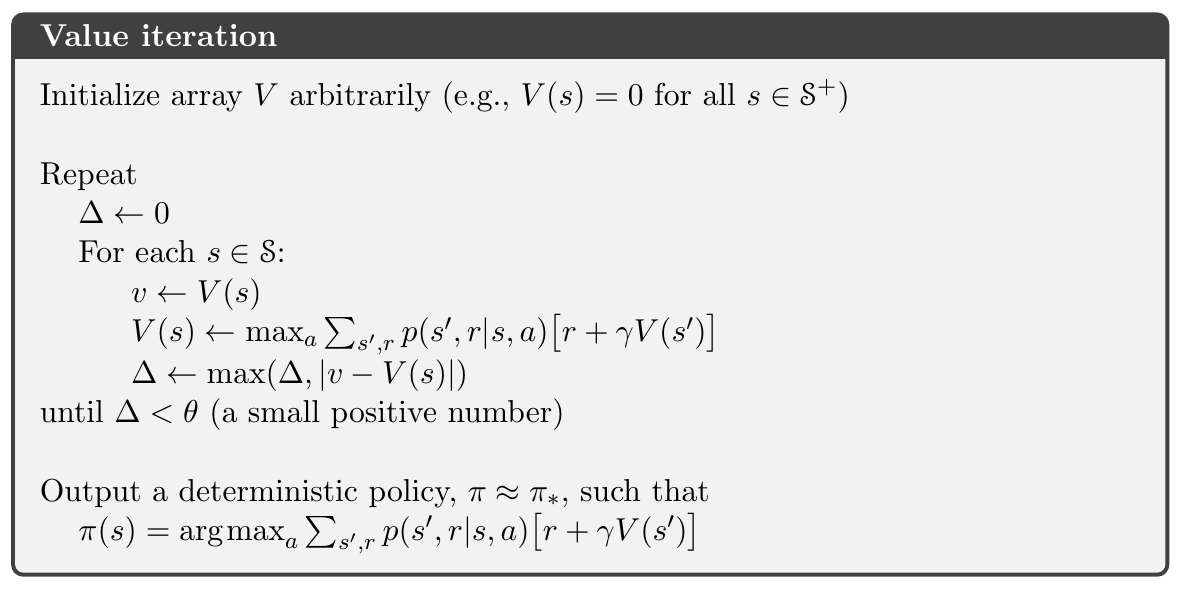
\includegraphics[scale=0.25]{value_iter_rl_intro_p92}
\end{figure}
\end{frame}

\begin{frame}
\frametitle{Dyna architecture}
\begin{figure}
    \centering
    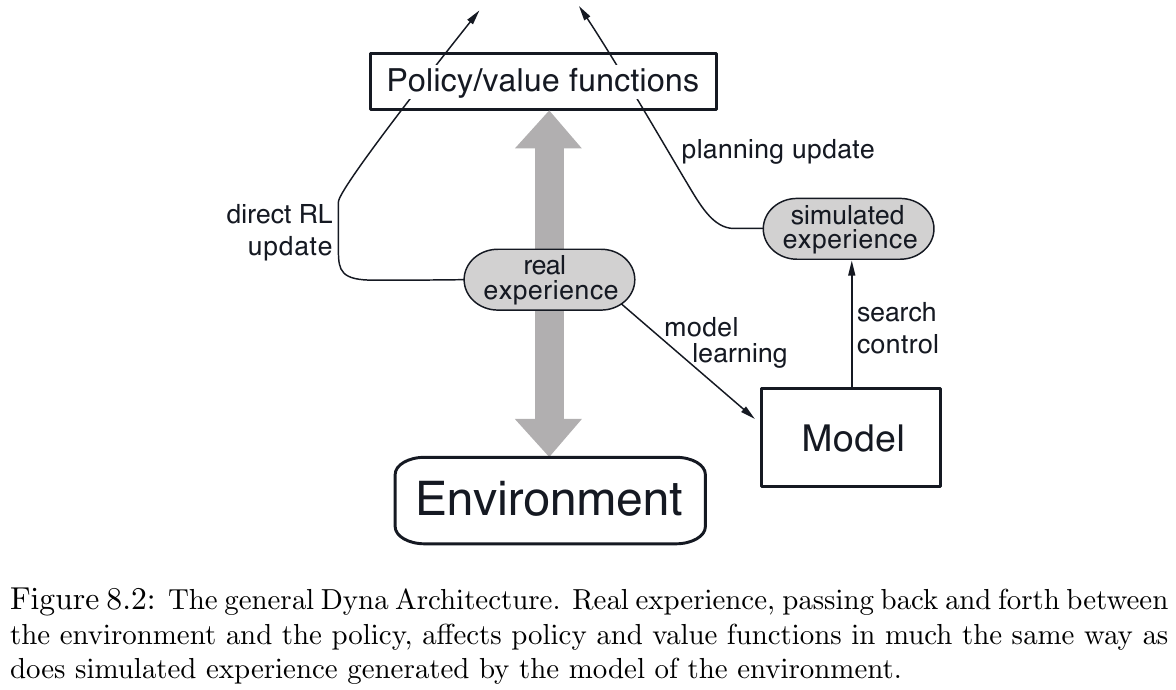
\includegraphics[scale=0.40]{dyna_rl_intro_p177}
\end{figure}
\end{frame}

\begin{frame}
\frametitle{Dyna algorithm}
\begin{figure}
    \centering
    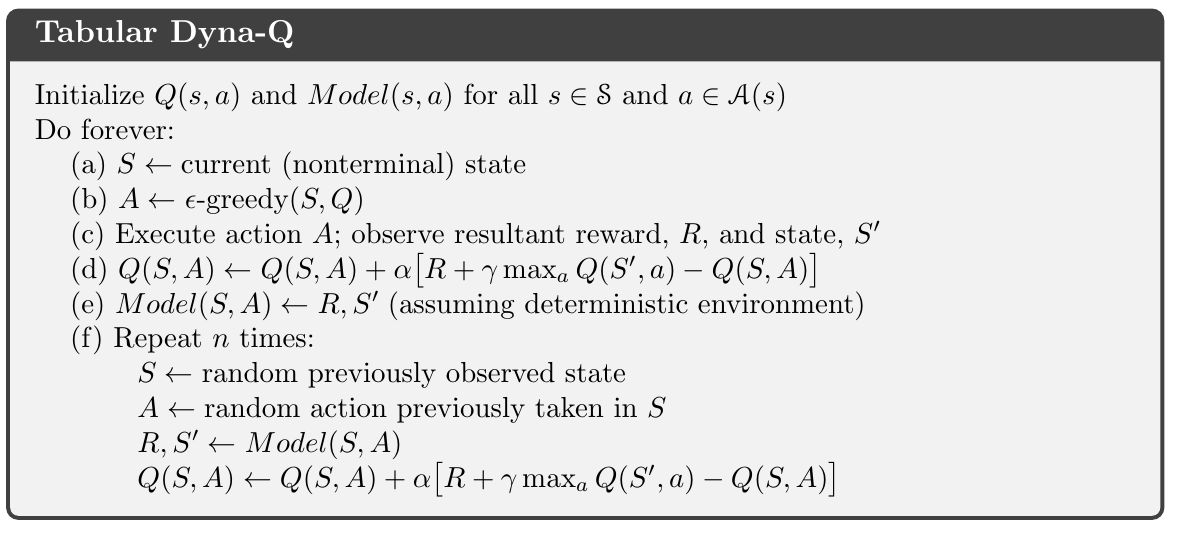
\includegraphics[scale=0.40]{dyna_algo_rl_intro_p178}
\end{figure}
\end{frame}

\begin{frame}
\frametitle{Dyna experiments}
\begin{figure}
    \centering
    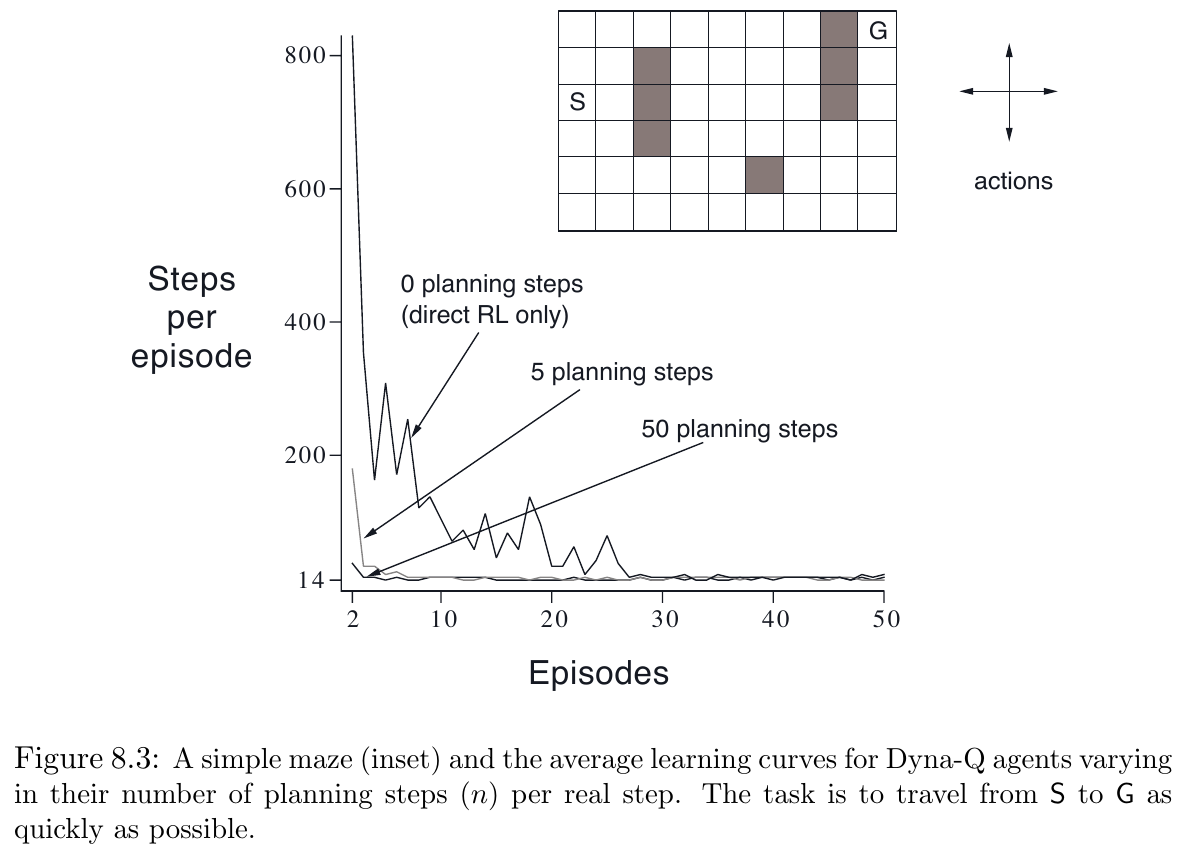
\includegraphics[scale=0.40]{dyna_plot_intro_p179}
\end{figure}
\end{frame}

\begin{frame}
\frametitle{Model learning as supervised and unsupervised learning}
\begin{figure}
    \centering
    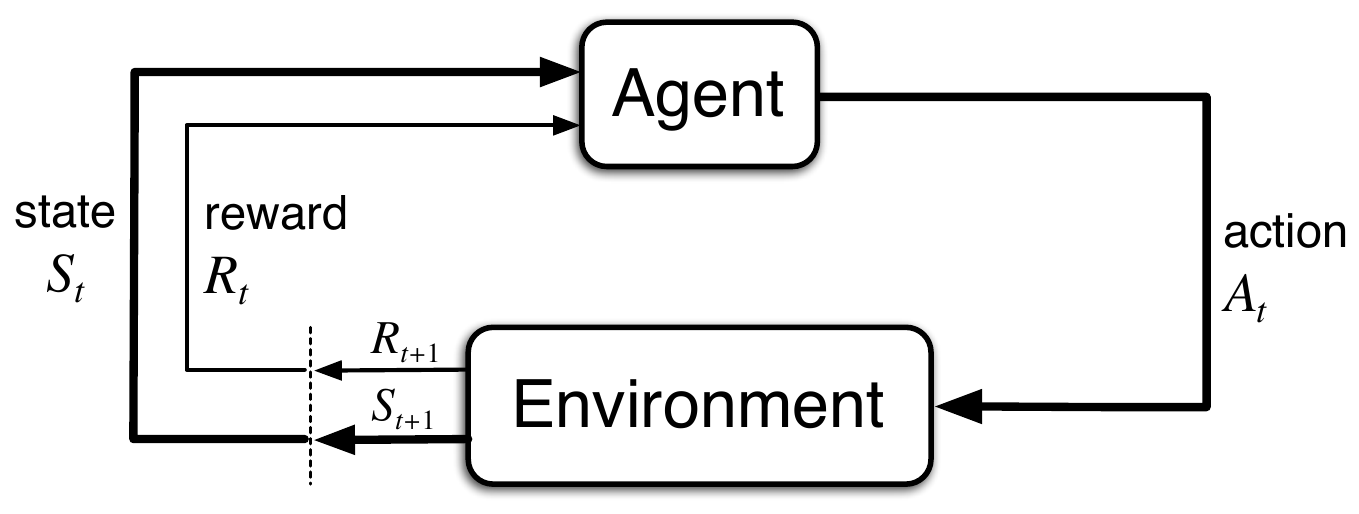
\includegraphics[scale=0.2]{agent_environment_rl_intro_p60}
\end{figure}

In model learning, \\
the goal is to estimate a model from experience, where:
$(S_1, A_1) \mapsto (S_2, R_2)$, \\
$(S_2, A_2) \mapsto (S_3, R_3)$,\\
\ldots,\\
$(S_{t-1}, A_{t-1}) \mapsto (S_t, R_t)$.
\vspace{2mm}
\pause

Thus, we have
\begin{itemize}
\item \textbf{regression} for the reward function, $(s, a) \mapsto r$
\item \textbf{density estimation} for the transition function, $(s, a) \mapsto s'$
\end{itemize}

\end{frame}

\begin{frame}
\frametitle{Changing (unstationary) Model}

Models may be incorrect because
\begin{itemize}
    \item the environment is stochastic and
    \item only a limited number of samples have been observed, or
    \item model was learned using function approximation
    \item the environment has changed
\end{itemize}

\end{frame}

\begin{frame}
\frametitle{Changing (unstationary) Model}

the Dyna agent with exploration bonus, Dyna-Q+,

% This
% agent keeps track for each state–action pair of how many time steps have elapsed since
% the pair was last tried in a real interaction with the environment. The more time that
% has elapsed, the greater (we might presume) the chance that the dynamics of this
% pair has changed and that the model of it is incorrect. To encourage behavior that
% tests long-untried actions, a special “bonus reward” is given on simulated experiences
% involving these actions. In particular, if the modeled reward for a transition is r,
% and the transition has not been tried in τ time steps, then planning backups are
% done as if that transition produced a reward of r + κ√
% τ , for some small κ.
\end{frame}

